\section{GAME PARTS}

\subsection{The Game Map}

The 17" by 22" mapsheet represents the battlefield at Hastings (actually Senlac Hill; Hastings is some miles to the south). The map is covered by a hexagonal grid to regulate movement and combat. The types of terrain and their effects are listed on the Terrain Effects Charts and in Section 5.3.

\subsection{The Playing Pieces}

The playing pieces, or counters, represent the forces (units) and commanders (leaders) involved in the battle. Certain other pieces (markers) are used to record unit status, time, and other game functions.

Historically, Williams's army included not only Normans, but Breton and Franco-Flemish contingents as well. Unless specifically stated otherwise, the term "Norman" refers to William's entire army.

\begin{center}
\textbf{Leader Units}
\end{center}
\par
\hspace{1em}
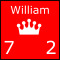
\includegraphics{Normans/William.jpg}
\hspace{1em}
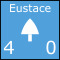
\includegraphics{Normans/Eustace.jpg}
\hspace{1em}
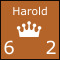
\includegraphics{Saxons/Harold.jpg}
\hspace{1em}
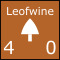
\includegraphics{Saxons/Leofwine.jpg}

\par
\begin{center}
  \textbf{Combat Units}
  \break
\end{center}

\renewcommand\tabularxcolumn[1]{m{#1}}
\begin{tabularx}{0.5\textwidth}{
    >{\raggedright\arraybackslash}X
    >{\centering\arraybackslash}X
    >{\raggedleft\arraybackslash}X}

  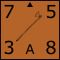
\includegraphics{Saxons/Housecarle.jpg} & \textbf{HouseCarles} & 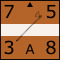
\includegraphics{Saxons/Housecarle_Ineffective.jpg} \\
  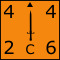
\includegraphics{Saxons/Thegn.jpg} & \textbf{Thegns} & 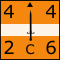
\includegraphics{Saxons/Thegn_Ineffective.jpg}
\end{tabularx}

\subsection{Game Charts and Tables}


The charts and tables simplify and illustrate certain game mechanics. These are the Norman and Saxon Order Tables, the Terrain Effects Chart, the Missile Fire Matrix, the Missile Fire Results Table, the Melee Results Table, the Morale Table, the Rally Table and the Leader Casualty Table. The locations and use of these charts and tables are noted in the appropriate rule sections.

\subsection{Game Tracks and Displays}

The tracks and displays used in the game are used to record unit status and the progress of the game. They include the Norman and Saxon Strategy Displays, the Norman and Saxon Order Displays, the Assault Period Display, the Battle Turn Record Track, and the Norman and Saxon Strategy Effect Tracks. These are located on the game map.

\subsection{Game Scale and Playing Time}

Each hex on the game map covers approximately 45 yards. Each housecarl or bowman unit represents about 100 men; all other units represent about 125-150 men. Each Assault Period should take from three to four hours to complete and covers several hours of real time. (Historians should note that the four separate phases of the actual battle have been reduced to two Assault Periods for play purposes.)

\subsection{Inventory of Game Parts}

A complete game includes:

\begin{enumerate}[label=*]
    \item One 17" x 22" game map
    \item One rule booklet
    \item 200 die-cut counters
\end{enumerate}

In addition, two six-sided dice must be provided by the players.